\documentclass[../main/main.tex]{subfiles}

\newdate{date}{30}{09}{2020}

% \begin{figure}[h!]
% \centering
% \includegraphics[page=6,width=0.8\textwidth]{../lessons/pdf_file/04_lecture.pdf}
% \end{figure}

%\displaydate{date}. Compiled:  \today. Alice.

\begin{document}

\pagestyle{plain}

\section{Lecture 4}


\subsubsection*{Slide 1}

\begin{minipage}[]{0.5\linewidth}
\centering
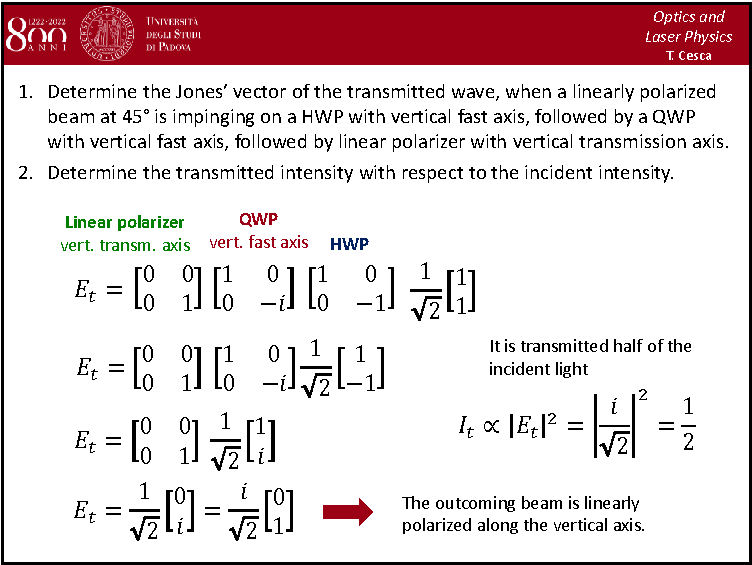
\includegraphics[page=1,width=1\textwidth]{../lessons/pdf_file/04_lecture.pdf}
\end{minipage}
\hspace{0.3cm}\vspace{0.3cm}
\begin{minipage}[c]{0.47\linewidth}
Let us this lecture with an exercise about the Jones'notation.

We need the amplitude of the trasmitted electric field. We are not using the simplified expression of the Jones's vector but also the amplitude factor to include it in the calculation.

For a half wave plate we do not have to specifcy the axis, it will be the same. For QWP it is important to specify that it has a vertical axis.

In the end we obtain the final vector, which is a linearly polarized beam along the vertical axis.

The intensity is proportional to the square modulus of the electric trasmitted field.

\end{minipage}

\subsubsection*{Slide 2}

\begin{minipage}[]{0.5\linewidth}
\centering
\includegraphics[page=2,width=1\textwidth]{../lessons/pdf_file/04_lecture.pdf}
\end{minipage}
\hspace{0.3cm}\vspace{0.3cm}
\begin{minipage}[c]{0.47\linewidth}

Let us talk about an incident beam impinging on an interface between two media with different refractive indexes. In the next slides, we will treat the interface as \textbf{planar} (in reality you have different shape, but you can think planar locally).

All we will demostrate comes from Maxwell equations. When we have a beam impinging on the interface, in order to guarantee the continuity of the component of the electric field, we have to consider a reflected beam and a trasmitted beam in the second medium.

It is easy to demostrate that we have a reflected beam which follow the \textbf{reflection law}:
\begin{equation*}
  \theta _i = \theta _r
\end{equation*}

\end{minipage}

Hence, one is the plane of the interface (perpendicular to the slide) and the incidence plane which contains the k vector of the incidents beam and normal to the interface (plane on the slide). Both the incident, relfected and trasmitted beam are \textbf{complanar}: they belong to the same incidence plane.

\subsubsection*{Slide 3}

\begin{minipage}[]{0.5\linewidth}
\centering
\includegraphics[page=3,width=1\textwidth]{../lessons/pdf_file/04_lecture.pdf}
\end{minipage}
\hspace{0.3cm}\vspace{0.3cm}
\begin{minipage}[c]{0.47\linewidth}

Another important law is the \textbf{Snell's law}, which gives you the relation between the incident and trasmitted beam. If \( n_2 > n_1 \), the trasmitted beam will stay to the normal to the interface with respewct to the incident beam. The opposite occurs if \( n_1 > n_2 \), you will have a trasmitted beam which forms a bigger angle. In this way, by measuring the angle, you can infer what is the medium which larger refractive index.

Having a larger refractive index means from an optical point of view that the medium is \emph{more dense}.

\end{minipage}

\newpage

\subsubsection*{Slide 4}

\begin{minipage}[]{0.5\linewidth}
\centering
\includegraphics[page=4,width=1\textwidth]{../lessons/pdf_file/04_lecture.pdf}
\end{minipage}
\hspace{0.3cm}\vspace{0.3cm}
\begin{minipage}[c]{0.47\linewidth}

There are different way to demostrate the previous law. A nice principle is the \textbf{Fermat's principle}, or lifeguard's principle. Which is the path that the lifeguard should do to reach the person as much as possible. We have an interface between two different media. It is easy to run in the sand than swimming in the water, hence sand is a medium with lower refractive index than water. The idea is that the lifeguard can do different path, which the shorter one is the one AB. However, the best path is the one travelled in the less time.

The \textbf{Fermat's principle idea} is that light select the path travelled in the shortest time.

\end{minipage}

There is an important consequence of this principle. If we are moving always in the same medium between point A and B, the questions is what is the best path to reach from A the point B? The best is the one travelled in the minimum time, which in this case is the straight line.
This is why we think light as rays.

To recap, we have to take the shortest path in time, not in space!

\subsubsection*{Slide 5}

\begin{minipage}[]{0.5\linewidth}
\centering
\includegraphics[page=5,width=1\textwidth]{../lessons/pdf_file/04_lecture.pdf}
\end{minipage}
\hspace{0.3cm}\vspace{0.3cm}
\begin{minipage}[c]{0.47\linewidth}

If you apply Snell's law at the two interfaces, from symmetry of the system you obtain the same angle at the ouput and the ray is shifted by a distance \( d \). The lateral shift can be related easily to the angles.
The shift can cause problems of alignments.

If you have a stack of materials with different refractive indexes, if you apply Snell's law to the interface and we are just interested in the angle at the output we can just consider the first and the last interface Snell's law relation. The intermediate steps are important if you want to calculate the lateral shift.

\end{minipage}

\subsubsection*{Slide 6}

\begin{minipage}[]{0.5\linewidth}
\centering
\includegraphics[page=6,width=1\textwidth]{../lessons/pdf_file/04_lecture.pdf}
\end{minipage}
\hspace{0.3cm}\vspace{0.3cm}
\begin{minipage}[c]{0.47\linewidth}

A consequence is the experiment of the broken spoon. Imagine to deep a spoon in a glass of water. We have air (\( n=1 \)) and water (\( n=1.33 \)). The ray will pass from two medium with different refractive indexes, so we will away the beam which is bending more.

\end{minipage}

\newpage

\subsubsection*{Slide 7}

\begin{minipage}[]{0.5\linewidth}
\centering
\includegraphics[page=7,width=1\textwidth]{../lessons/pdf_file/04_lecture.pdf}
\end{minipage}
\hspace{0.3cm}\vspace{0.3cm}
\begin{minipage}[c]{0.47\linewidth}

Another example is related to the sunset. When you see the sun, the sun is already below the horizont and you are able to see it in an apparent position. This is why the refractive index of the atmosphere (of a medium in general) increases with density and decreases with temperature at a given altitude. If the refractive indexes increases with density, it means that the closer you have the ray of light to the earth, more dense will be the atmosphere and so the higher will be the refractive index. This means that the beam is bending toward the normal at the earth and you have a continuous bending of your ray. This can lead to different of several minutes like 2-3 minutes.
\end{minipage}

In the opposite way, you can explain with the same idea the fact that in very hot days you have the feeling that the asphalt is with water. You are just seeing the reflection of the sky. This is due to the fact that the refractive index decreases with temperature at a given altitude. In this case we have a ray which is entering the atmosphere and if the earth is very hot, the ray will be bent far away from the normal. You will have the apparence of reflecting surface like water, but it is just the reflection of the sky.

\subsubsection*{Slide 8}

\begin{minipage}[]{0.5\linewidth}
\centering
\includegraphics[page=8,width=1\textwidth]{../lessons/pdf_file/04_lecture.pdf}
\end{minipage}
\hspace{0.3cm}\vspace{0.3cm}
\begin{minipage}[c]{0.47\linewidth}

Another example is the deviation in a triangular prism: this is a geometrical exercise. The angle of minimum deviation is the angle for which the output angle is the same as the incidence angle. In this case you are in the condition of \textbf{minimum deviation}.

The important things is that the refractive index is \emph{dependent on the wavelength}. So any material we are considering have a \textbf{dispersion}.

\end{minipage}

\subsubsection*{Slide 9}

\begin{minipage}[]{0.5\linewidth}
\centering
\includegraphics[page=9,width=1\textwidth]{../lessons/pdf_file/04_lecture.pdf}
\end{minipage}
\hspace{0.3cm}\vspace{0.3cm}
\begin{minipage}[c]{0.47\linewidth}

So, if you are in the condition of minimum deviation and considering that the refractive index depends on the wavelength, if you imping in the triangular prism with a white beam (so all the components at different wavelength) you will end up with the spread of the different wavelengths at different angles.

The refractive index is minimum for infrared and gets larger towards ultraviolet. So you will have a spread minimum for the red color and larger going to the violet. Prism can be used as a way to separate the colors as Newton shown.

\end{minipage}

\subsubsection*{Slide 10}

\begin{minipage}[]{0.5\linewidth}
\centering
\includegraphics[page=10,width=1\textwidth]{../lessons/pdf_file/04_lecture.pdf}
\end{minipage}
\hspace{0.3cm}\vspace{0.3cm}
\begin{minipage}[c]{0.47\linewidth}

This image contains a lot of informations about what you see when the rainbow forms. We have the \textbf{primary} and \textbf{secondary} \textbf{arch}. The bend bwteen the two arch is darker (\textbf{Alessandro's dark band}). There is also a \textbf{bright band} below the primary arch. Moreover, the colors in the primary and secondary arch are reversed.


\end{minipage}

\subsubsection*{Slide 11}

\begin{minipage}[]{0.5\linewidth}
\centering
\includegraphics[page=11,width=1\textwidth]{../lessons/pdf_file/04_lecture.pdf}
\end{minipage}
\hspace{0.3cm}\vspace{0.3cm}
\begin{minipage}[c]{0.47\linewidth}

We can apply the property of the dispersion and polarization. The main idea is that a rainbow is formed when you have water drops in the atmosphere and reflection of sun light of the water drops. We have two different angles for the two archs.

\end{minipage}

\subsubsection*{Slide 12}

\begin{minipage}[]{0.5\linewidth}
\centering
\includegraphics[page=12,width=1\textwidth]{../lessons/pdf_file/04_lecture.pdf}
\end{minipage}
\hspace{0.3cm}\vspace{0.3cm}
\begin{minipage}[c]{0.47\linewidth}

We have a ray that is impinging inside the water drop. The ray is reflected outside and refracted inside and so on. If you consider the angle of minimum deviation it is easy to demonstrate that it is 138°.

\end{minipage}

\subsubsection*{Slide 13}

\begin{minipage}[]{0.5\linewidth}
\centering
\includegraphics[page=13,width=1\textwidth]{../lessons/pdf_file/04_lecture.pdf}
\end{minipage}
\hspace{0.3cm}\vspace{0.3cm}
\begin{minipage}[c]{0.47\linewidth}

The secondary arch is created when light enters the drop in the bottom part and makes two reflections inside the drop.

So, the primary arch is formed by rays that are reflected just one in the water drop, while the secondary arch is formed by the rays that are reflected two times inside the water drop.

If you consider the dispersion law, you can demonstrated the dispersion of the different colors and that the colors are reversed for the two arch.


\end{minipage}

\subsubsection*{Slide 14}

\begin{minipage}[]{0.5\linewidth}
\centering
\includegraphics[page=14,width=1\textwidth]{../lessons/pdf_file/04_lecture.pdf}
\end{minipage}
\hspace{0.3cm}\vspace{0.3cm}
\begin{minipage}[c]{0.47\linewidth}

To see the formation of two bright spots near the sun you have to be in a cold place. We can see the dispersion of the different colors.

\end{minipage}

\subsubsection*{Slide 15}

\begin{minipage}[]{0.5\linewidth}
\centering
\includegraphics[page=15,width=1\textwidth]{../lessons/pdf_file/04_lecture.pdf}
\end{minipage}
\hspace{0.3cm}\vspace{0.3cm}
\begin{minipage}[c]{0.47\linewidth}

The last phenomena is related to refraction inside the ice place (this is why we can see \textbf{sun dogs} in place where the atmosphere is cold in which you can think of having also ice). As for the triangular prism, we can calculate the angle of minimum deviation.

\end{minipage}

\subsubsection*{Slide 16}

\begin{minipage}[]{0.5\linewidth}
\centering
\includegraphics[page=16,width=1\textwidth]{../lessons/pdf_file/04_lecture.pdf}
\end{minipage}
\hspace{0.3cm}\vspace{0.3cm}
\begin{minipage}[c]{0.47\linewidth}

Beam impinging on an interface between two different media. We start to take into account also the amplitude of the electric field and magnetic field. As we have seen, we have different polarization waves. Actually, we can describe every polarization state as superposition of two components of two linearly polarized wave along ortoghonal direction with a phase shift.

\textbf{Transverse Electric (TE) polarization} to describe linearly polarized way in which electric field is perpendicular to the plane of incidence (when we talk about polarization we refer to the polarization of the electric field!). Hence, the electric field is parallel to the plane of the interface.


\end{minipage}

\subsubsection*{Slide 17}

\begin{minipage}[]{0.5\linewidth}
\centering
\includegraphics[page=17,width=1\textwidth]{../lessons/pdf_file/04_lecture.pdf}
\end{minipage}
\hspace{0.3cm}\vspace{0.3cm}
\begin{minipage}[c]{0.47\linewidth}

\textbf{Transverse Magnetic (TM) polarization}, i.e. the electric field is parallel to the plane of incidence. If the electric field is parallel, the magnetic field is perpendicular to the incidence plane.

The choice about orienting the electric field (and consequently the magnetic field) is simply a convention. This convention is motivated by a physical meaning, but you can find in any books a different orientation. Physically, the difference are only related to the orientation of the electric field for the reflected beam when you consider TM. In many books you can find the same convention for the TE but a different one for the TM.

\end{minipage}

\subsubsection*{Slide 18}

\begin{minipage}[]{0.5\linewidth}
\centering
\includegraphics[page=18,width=1\textwidth]{../lessons/pdf_file/04_lecture.pdf}
\end{minipage}
\hspace{0.3cm}\vspace{0.3cm}
\begin{minipage}[c]{0.47\linewidth}

The reason of the convention is the following. Let us consider the situation in which we are at \textbf{normal incidence} in which TE and TM are degenerate (exaclty the same). You are not able to distinguish them at normal incidence. So you cannot use the orientation of electric and magnetic field to distinguish them.

If you do the same with the opposite convention, you can immediatly see that in this case you can distinguish the two polarizations. This is a none sense physically.

\end{minipage}



\end{document}
